\documentclass[dvipdfmx,12pt]{beamer}
\usepackage{bxdpx-beamer}
\usepackage{pxjahyper}
\usepackage{tikz}
\usepackage{here}
\usepackage{graphicx}
\renewcommand{\kanjifamilydefault}{\gtdefault}

\usepackage{amsmath}
\usepackage{amsfonts}
\usepackage{amssymb}
\usepackage{color}
\usepackage{tcolorbox}
\usepackage{forest}

\usetikzlibrary{arrows.meta}
\usetikzlibrary{positioning}

\usetheme{metropolis}  

% blockのスタイルをカスタマイズ
\setbeamercolor{block title}{bg=blue!30,fg=black} % タイトルの背景色とテキストの色
\setbeamercolor{block body}{bg=blue!10,fg=black} % ボディの背景色とテキストの色

\usepackage[usetype1]{uline--}

\title{第3回MPC勉強会}
\author{鶴原康太}

\begin{document}

    \frame{\maketitle}
    
    \begin{frame}{今回の目標}
        \footnotesize
        HJB方程式を理解する
        \begin{equation*}
            -\frac{\partial V}{\partial t}\left(x,t\right) = \min _u H\left(x, u, \left( \frac{\partial V}{\partial x} \right)^T\left(x, t\right), t \right)
        \end{equation*}
        \centering
    \end{frame}

    \begin{frame}{前回のおさらい}
        微分法 \\

        変分法 \\

        偏微分と似た考え方をする \\

        二点境界値問題の解 \\
        オイラーラグランジュ方程式を満たす \\
        制約を含んだ場合 \\
    \end{frame}

    \begin{frame}{最適性条件まとめ}
        \footnotesize
        ラグランジュの未定乗数法\\
        KKT条件\\
        オイラーラグランジュ方程式\\
    \end{frame}

    \begin{frame}{動的計画法1}
        \footnotesize
        \begin{align*}
            \dot{x}(t) &= f(x(t), u(t), t) \\
            H(x, u, \lambda, t) &= L(x, u, t) + \lambda^T f(x, u, t) \\
            J &= \psi(x(t_f)) + \int_{t_0}^{t_f} L(x(t), u(t), t) \, dt
        \end{align*}
    
        別の表現を見てみる
    
        \begin{align*}
            V(x, t) = \min_{u[t, t_f]} \left( \psi(x(t_f)) + \int_t^{t_f} L(x(\tau), u(\tau), \tau) d\tau \right)
        \end{align*}
    
        \begin{align*}
            V(x, t) = \min_{u[t, t_f]} \left( \int_t^{t+dt} L(x(\tau), u(\tau), \tau) d\tau + \psi(x(t_f)) + \int_{t+dt}^{t_f} L(x(\tau), u(\tau), \tau) d\tau \right)
        \end{align*}

        \begin{align*}
            V(x, t) &= \min_{u[t, t+dt]} \left( \int_t^{t+dt} L(x(\tau), u(\tau), \tau) d\tau + \min_{u[t+dt, t_f]} \left( \psi(x(t_f)) + \int_{t+dt}^{t_f} L(x(\tau), u(\tau), \tau) d\tau \right) \right) \\
            &= \min_{u[t, t+dt]} \left( \int_t^{t+dt} L(x(\tau), u(\tau), \tau) d\tau + V \left( x + \int_t^{t+dt} f(x, u, \tau) d\tau, t + dt \right) \right) \\
            &= \min_u \left( L(x, u, t) dt + V \left( x + f(x, u, t) dt, t + dt \right) \right)
        \end{align*}

        次元の呪い
    
    \end{frame}

    \begin{frame}{動的計画法2}
        \begin{figure}[H]
            \centering
            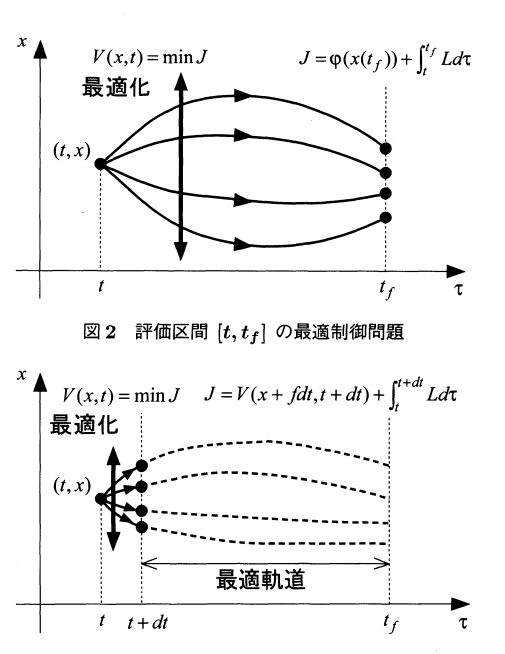
\includegraphics[clip, width = 4.0cm]{DP.png}
        \end{figure}
        \centering
        \tiny{
            \rightline{
                大塚:非線形最適制御入門
            }
        }
    \end{frame}
    
    \begin{frame}{動的計画法3}
        \footnotesize
    \end{frame}

    \begin{frame}{HJB方程式}
        \footnotesize
        
        \begin{align*}
            H(x, u, \lambda, t) &= L(x, u, t) + \lambda^T f(x, u, t) \\
            -\frac{\partial V}{\partial t}\left(x,t\right) = \min _u H\left(x, u, \left( \frac{\partial V}{\partial x} \right)^T\left(x, t\right), t \right)
        \end{align*}
        \centering
        次元の呪い\\
    \end{frame}

    \begin{frame}{Pontryaginの最小原理}
        \footnotesize

    \end{frame}

    \begin{frame}{最適性条件まとめ}
        \footnotesize
        ラグランジュの未定乗数法\\
        KKT条件\\
        オイラーラグランジュ方程式\\
        動的計画法(new)\\
        HJB方程式(new)\\
        最小原理(new)\\
        動的計画法からHJB方程式を導いたが、最小原理からも導ける\\

        ここに各関係の図を貼る
    \end{frame}

    \begin{frame}{参考資料}
        \footnotesize

        書籍\\
        \begin{itemize}
            \item 非線形最適制御入門(名著です)
            \item しっかり学ぶ数理最適化(最適化全般について)
            \item はじめての最適化(変分法の説明が分かりやすいです)
        \end{itemize}

        サイト(URL) \\
        \begin{itemize}
            \item MyEnigmaのMPC導入: \href{https://myenigma.hatenablog.com/entry/2016/07/25/214014}{https://myenigma.hatenablog.com/entry/2016/07/25/214014}
            \item MyEnigmaのMPC数式: \href{https://myenigma.hatenablog.com/entry/2017/02/07/084922}{https://myenigma.hatenablog.com/entry/2017/02/07/084922}
            \item MPCの具体例: \href{https://ramune6110.hatenablog.com/entry/2022/02/13/154405}{https://ramune6110.hatenablog.com/entry/2022/02/13/154405}
            \item MPCを用いた倒立振子: \href{https://qiita.com/slowsingle/items/f3074ea6670da42696e0}{https://qiita.com/slowsingle/items/f3074ea6670da42696e0}
            \item MPCの説明と実機を用いた実験: \href{http://www.kostasalexis.com/linear-model-predictive-control.html}{http://www.kostasalexis.com/linear-model-predictive-control.html}
        \end{itemize}
    \end{frame}
    
\end{document}